%! Author = kubec
%! Date = 27.03.2024

% Preamble
\documentclass[11pt]{article}

% Packages
\usepackage{amsmath}
\usepackage{mathtools}
\usepackage{ragged2e}
\usepackage [utf8]{inputenc}
\usepackage{blindtext}
\usepackage{wrapfig}
\usepackage{xcolor}
\usepackage {polski}
\usepackage{multicol}
\usepackage[a4paper, total={5.7in, 8in}]{geometry}
\usepackage{graphicx}
\usepackage{amstex}
\usepackage{csvsimple}
\usepackage{changepage}
\usepackage{enumitem}
\usepackage[english]{babel}
\usepackage{biblatex}
\usepackage{caption}
\usepackage{indentfirst}

\newenvironment{changemargin}[2]{%
    \begin{list}{}{%
        \setlength{\topsep}{0pt}%
        \setlength{\leftmargin}{#1}%
        \setlength{\rightmargin}{#2}%
        \setlength{\listparindent}{\parindent}%
        \setlength{\itemindent}{\parindent}%
        \setlength{\parsep}{\parskip}%
    }%
        \item[]}{\end{list}}

% Document
\begin{document}
    \begin{flushright}
        \large{
            Igor Czerwiec - 277680\\
            Filip Kubecki - 272655
        }\\
    \end{flushright}
    \begin{center}
        \large{Fizyka 3.1}\\
        \vspace{2mm}
        \LARGE{\textbf{Wyznaczanie współczynnika rozszerzalności termicznej oraz badanie procesów przekazywania ciepła}}\\
        \vspace{3mm}
        \huge{Nr ćwiczenia: 29}\\
        \vspace{1cm}
    \end{center}
    \begin{flushright}
        \large{
            Data wykonania ćwiczenia: 18.04.2024 r.\\
            Data oddania sprawozdania: 25.04.2024 r.
        }\\
    \end{flushright}
    \vspace{1cm}
    \section{Wstęp}
    \textbf{Wykorzystane przyrządy pomiarowe:}
    \begin{itemize}
        \itemsep0em
        \item Termometr cyfrowy YCT YC-61N
        \item Zasilacz prądu stałego Zhaoxin RXN-1505D
        \item Czujnik mikrometryczny (o dokładności $\pm$1 [${\mu}m$])
    \end{itemize}
    \subsection*{Przebieg doświadczenia}
    Doświadczenie polegało na stopniowym podgrzewaniu drutu umieszczonego w specjalnej obudowe ogarniczającej utratę ciepła.
    Podgrzewanie odbywało się poprzez
    zwiększanie różnicy potencjałów na końcach drutu. Zasilacz zasilający układ był cały czas nastawiony na maksymalny prąd (brak ogarniczenia prądowego).
    W trakcie doświadczenia notowano kolejno wartości prądu, napięcia, wydłużenia drutu oraz temperatury drutu.\\
    \indent Po nagrzaniu drutu do temperatury maksymalnej (150 [${^\circ}C$]) z obudowy wyciągnięto przednią ściankę. Następnie powtórzono doświadczenie
    powoli schładzając drut poprzez obniżanie napięcia podawanego na niego. Pomiary powtarzano aż do temperatury pokojowej.
    
    \section{Obliczenia}
    \noindent Niepewność termometru wyznaczono ze wzoru podanego przez producenta:
    \begin{gather*}
        u(t)=0.05\%\cdot rdg+0.5\cdot res
    \end{gather*}
    {\footnotesize
        \begin{itemize}
            \item[] $rdg$ - wartość odczytana,
            \item[] $res$ - rozdzielczość zakresu,
        \end{itemize}}
    \noindent Przykładowo:
    \begin{gather*}
        u(t)=0.05\%\cdot 24.1[^{\circ}C]+0.5\cdot 0.1=0.06205 [^{\circ}C]\approx 0.063 [^{\circ}C]
    \end{gather*}
    \noindent Niepewność pomiaru temperatury wyliczono ze wzoru na niepewność standardową typu B:
    \begin{gather*}
        u_b(t)=\sqrt{\frac{u^2(t)}{3}+\frac{\Delta_{eks}^2}{3}+\frac{\Delta_{st}^2}{3}}
    \end{gather*}
    {\footnotesize
        \begin{itemize}
            \item[] $u(t)$ - niepewność pomiarowa termometru,
            \item[] $\Delta_{eks}$ - niepewność odczytu eksprymentatora,
            \item[] $\Delta_{st}$ - niepewność wynikająca ze stabilizacji temperatury,
        \end{itemize}}
    \noindent Przykładowo:
    \begin{gather*}
        u_b(t)=\sqrt{\frac{0.06205^2}{3}+\frac{0.1^2}{3}+\frac{0.2^2}{3}}=0.133977862 [^{\circ}C]\approx 0.14 [^{\circ}C]
    \end{gather*}
    \noindent Niepewność pomiaru długości została wyliczona ze wzoru na niepewność standardową typu B:
    \begin{gather*}
        u_b(t)=\sqrt{\frac{u^2(L)}{3}}
    \end{gather*}
    {\footnotesize
        \begin{itemize}
            \item[] $u(L)$ - niepewność mikrometra,
        \end{itemize}}
    \noindent Przykładowo:
    \begin{gather*}
        u_b(L)=\sqrt{\frac{1^2[\mu m]}{3}}=0.577350269 [\mu m]\approx 0.58 [\mu m]
    \end{gather*}
    \noindent Niepewność obliczenia $\frac{\Delta L}{L_0}$ wyliczono ze wzoru na niepewność złożoną:
    \begin{gather*}
        u_c(\frac{\Delta L}{L_0})=\sqrt{(\frac{\partial \frac{\Delta L}{L_0}}{\partial \Delta L}+u(\Delta L))^2+(\frac{\partial \frac{\Delta L}{L_0}}{\partial L_0}+u(L_0))^2}
    \end{gather*}
    \noindent Przykładowo:
    \begin{gather*}
        u_c(\frac{\Delta L}{L_0})=\sqrt{(\frac{1}{0.875 [m]}\cdot 0.58[\mu m])^2+(\frac{2[\mu m]}{0.875^2[\mu m]}\cdot 0.002309401[m])^2}=\\
        =6.59856\cdot 10^{-7} [m]\approx 6.6\cdot 10^{-7} [m]
    \end{gather*}
    \noindent Moc wyliczono ze wzoru:
    \begin{gather*}
        P=U\cdot I
    \end{gather*}
    \noindent Przykładowo:
    \begin{gather*}
        P=5[V]\cdot 1.2[A]=6[W]
    \end{gather*}
    \noindent Niepewność obliczenia mocy wyliczono ze wzoru na niepewność złożoną:
    \begin{gather*}
        u_c(P)=\sqrt{(\frac{\partial P}{\partial U}\cdot u(U))^2+((\frac{\partial P}{\partial I}\cdot u(I))^2}=\\
        =\sqrt{(I\cdot u(U))^2+(U\cdot u(I))^2}
    \end{gather*}
    \noindent Przykładowo:
    \begin{gather*}
        u_c(P)=\sqrt{(1[A]\cdot 0.058[V])^2+(4.2[V]\cdot 0.058[A])^2}\approx 0.25 [W]
    \end{gather*}
    \noindent Niepewności prądu i napięcia zostały wyliczone ze wzoru na niepewność standardową typu B przy założeniu że dokładność odczytu wynosi 0.1 jednostki.

    \section{Dane oraz wyniki}
    \subsection*{Współczynnik rozszerzalności}
    \begin{center}
        Tabela 1 - podgrzewanie z włożoną szybką
    \end{center}
    \begin{center}
        \csvreader[tabular = |c|c|c|c|c|c|c|,
            table head = \hline \textbf{$L_0$[m]} & \textbf{$t_0$[${^\circ}C$]} & \textbf{$t$[${^\circ}C$]} &
            \textbf{$\Delta t$[${^\circ}C$]} & \textbf{$\Delta L$[${\mu}m$]} & \textbf{$\frac{\Delta L}{L_0}$[${\mu}m$]} & \textbf{(u$\frac{\Delta L}{L_0})$[${\mu}m$]} \\\hline,
            late after line = \\\hline
        ]{Dane/Wyniki1.csv}{}{
            \csvcoli & \csvcolii & \csvcoliii & \csvcoliv & \csvcolv & \csvcolvi & \csvcolvii
        }
    \end{center}
    Współczynnik temperaturowy:
    \begin{gather*}
        \alpha=1.457\pm 0.040 [10^{-6}\cdot K^{-1}]
    \end{gather*}
    Wykres zależności zmiany długości od zmiany temperatury:
    \begin{center}
        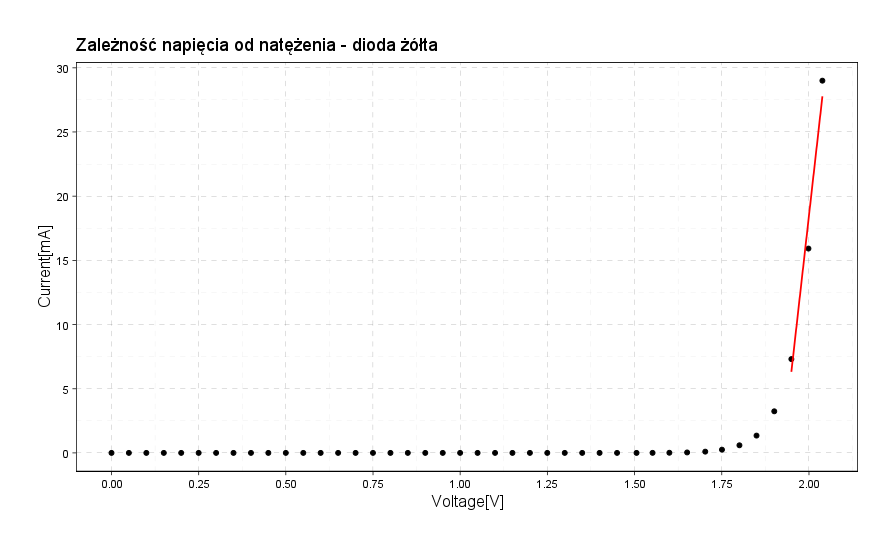
\includegraphics[scale = 0.5]{"F:/Projekty Intellij/Text/Fizyka3.1/29/Img/Rplot01.png"}
    \end{center}
    \textbf{Uwaga} - na wykresie zostały zamieszczone pola niepewności. Jednak z powodu bardzo niewielkich błędów pomiarowych
    pola niepewności wyglądają jak ledwo widoczne czerwone kropki wewnątrz punktów oznaczających kolejne pomiary.
    \\
    \begin{center}
        Tabela 2 - Ochładzanie z wyciągniętą szybką
    \end{center}
    \begin{center}
        \csvreader[tabular = |c|c|c|c|c|,
            table head = \hline \textbf{$t$[${^\circ}C$]} &
            \textbf{$\Delta t$[${^\circ}C$]} & \textbf{$\Delta L$[${\mu}m$]} & \textbf{$\frac{\Delta L}{L_0}$[${\mu}m$]} & \textbf{(u$\frac{\Delta L}{L_0})$[${\mu}m$]} \\\hline,
            late after line = \\\hline
        ]{Dane/Wyniki2.csv}{}{
            \csvcoli & \csvcolii & \csvcoliii & \csvcoliv & \csvcolv
        }
    \end{center}
    Współczynnik temperaturowy:
    \begin{gather*}
        \alpha=1.570\pm 0.020[10^{-6}\cdot K^{-1}]
    \end{gather*}
    Wykres zależności zmiany długości od zmiany temperatury:
    \begin{center}
        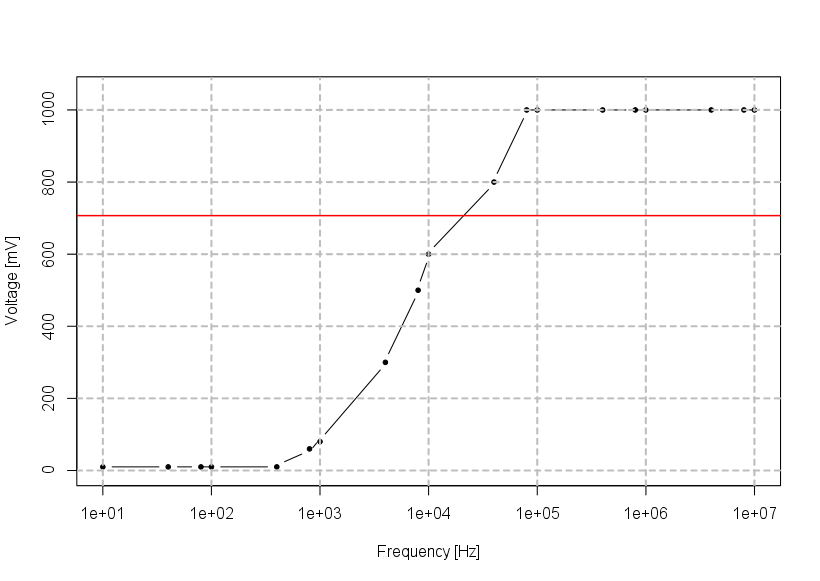
\includegraphics[scale = 0.5]{"F:/Projekty Intellij/Text/Fizyka3.1/29/Img/Rplot02.png"}
    \end{center}
    \textbf{Uwaga} - na wykresie zostały zamieszczone pola niepewności. Jednak z powodu bardzo niewielkich błędów pomiarowych
    pola niepewności wyglądają jak ledwo widoczne czerwone kropki wewnątrz punktów oznaczających kolejne pomiary.
    
    \subsection*{Moc}
    \begin{center}
        Tabela 3 - podgrzewanie z włożoną szybką
    \end{center}
    \begin{center}
        \csvreader[tabular = |c|c|c|c|c|c|c|,
            table head = \hline \textbf{\boldmath$t_0$[${^\circ}C$]} & \textbf{I[A]} & \textbf{U[V]} &
            \textbf{P[W]} & \textbf{u(P)[W]} & \textbf{T[${^\circ}C$]} &
            \textbf{${\Delta}T$[${^\circ}C$]} \\\hline,
            late after line = \\\hline
        ]{Dane/Wyniki3.csv}{}{
            \csvcoli & \csvcolii & \csvcoliii & \csvcoliv & \csvcolv & \csvcolvi & \csvcolvii
        }
    \end{center}
    Wykres zależności mocy od zmiany temperatury:
    \begin{center}
        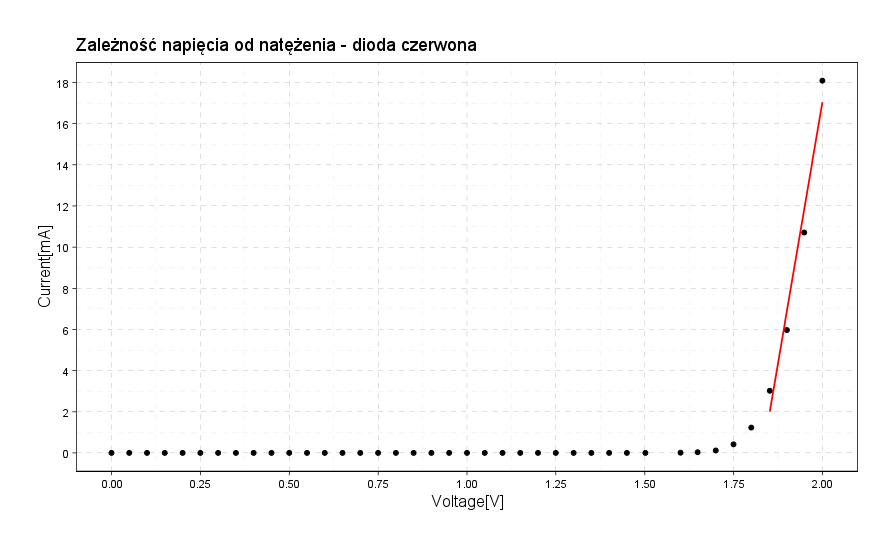
\includegraphics[scale = 0.5]{"F:/Projekty Intellij/Text/Fizyka3.1/29/Img/Rplot03.png"}
    \end{center}
    \\
    \begin{center}
        Tabela 4 - ochładzanie z wyciągniętą szybką
    \end{center}
    \begin{center}
        \csvreader[tabular = |c|c|c|c|c|c|c|,
            table head = \hline \textbf{\boldmath$t_0$[${^\circ}C$]} & \textbf{I[A]} & \textbf{U[V]} &
            \textbf{P[W]} & \textbf{u(P)[W]} & \textbf{T[${^\circ}C$]} &
            \textbf{${\Delta}T$[${^\circ}C$]} \\\hline,
            late after line = \\\hline
        ]{Dane/Wyniki4.csv}{}{
            \csvcoli & \csvcolii & \csvcoliii & \csvcoliv & \csvcolv & \csvcolvi & \csvcolvii
        }
    \end{center}\newpage
    Wykres zależności mocy od zmiany temperatury:
    \begin{center}
        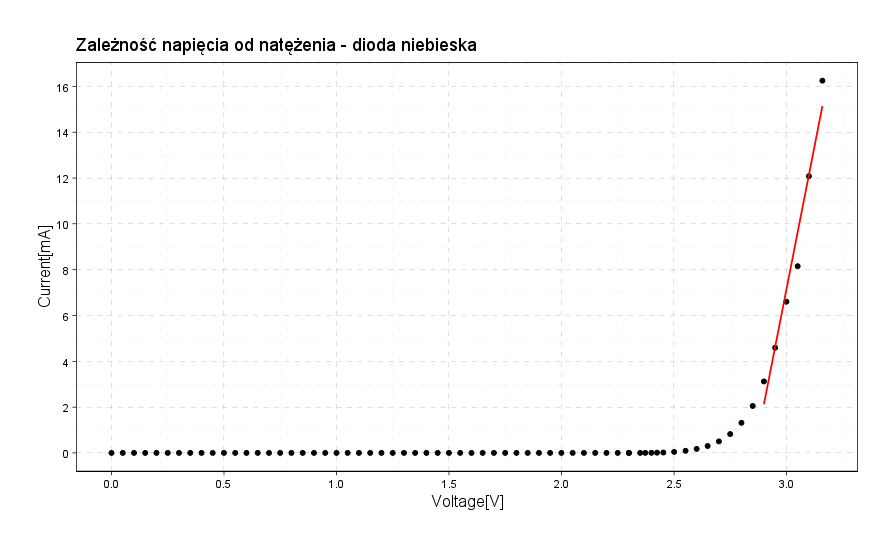
\includegraphics[scale = 0.5]{"F:/Projekty Intellij/Text/Fizyka3.1/29/Img/Rplot04.png"}
    \end{center}

    \newpage
    \section{Wnioski}
    Na podstawie pierwszej części ćwiczenia wyznaczono współczynniki rozszerzalności materiału z którego został wykonany drut:
    \begin{gather*}
        \alpha=1.457\pm 0.040 [10^{-6}\cdot K^{-1}]\\
        \alpha=1.570\pm 0.020[10^{-6}\cdot K^{-1}]
    \end{gather*}
    \indent Na podstawie tych wyników jesteśmy w stanie wywnioskować że drut został prawdopodobnie wykonany z Inwaru (stop żelaza i niklu - FeNi36)
    dla którego wartość tego współczynnika waha się według różnych danych w przedziale od $1.3[10^{-6}\cdot K^{-1}]$ do $1.5[10^{-6}\cdot K^{-1}]$.
    Można więc wnioskować że ta część zadania została przeprowadzona poprawnie.\\

    W drugiej części zadania wyznaczono charakterystykę mocy od zmiany temperatury dla druta podgrzewanego z zamkniętą komorą oraz otwartą komorą.
    Z powodu pomiaru prądu oraz napięcia zasilacza przy pomocy niedokładnych indykatorów wbudowanych w zasilacz nie udało się dokładnie wyznaczyć
    charakterystyki. Nieliniowość tej zależności jest mało widoczna na wykresach. Również różnice między mocami w przypadku otwartej oraz zamkniętej komory
    są zauważalne dopiero przy porównaniu danych w tabelach. Może to być również spowodowane błędnym przeprowadzeniem drugiej części doświadczenia
    (schładzania od temperatury maksymalnej do pokojowej zamiast wychłodzić drut a następnie ponownie podgrzewać go bez szybki).\\
    \indent Nie powstrzymuje to nas jednak od wyciągnięcia wniosków zleconych w karcie zadania. Wykresy zależności mocy od zmiany temperatury
    nie powinny być wykresami liniowymi ze względu na zjawisko wymiany ciepła, działające na ciała o różnych temperaturach. W tym wypadku ciało
    oddaję temperaturę do otoczenia, gdzie im wyższa różnica temperatur tym większa wymiana ciepła. Skutkuje to wzrostem wymaganej mocy do podgrzania ciała
    wraz ze wzrostem temperatury. Przy otwartej szybie zapotrzebowanie na moc jest większe gdyż zwiększamy dostęp do materii z którą drut może wymienić
    się energią.

    %Bibliografia
    \vfill
    \footnotesize
    \begin{thebibliography}{9}
        \bibitem{texbook1}
        https://lpf.wppt.pwr.edu.pl/instrukcje/cwn029.pdf
        \bibitem{texbook2}
        https://lpf.wppt.pwr.edu.pl/pomoce-dydaktyczne.php
        \bibitem{texbook3}
        https://www.wolframalpha.com/
        \bibitem{texbook4}
        https://www.engineeringtoolbox.com/linear-expansion-coefficients-d-95.html
        \bibitem{texbook5}
        https://en.wikipedia.org/wiki/Invar
        \bibitem{texbook6}
        https://en.wikipedia.org/wiki/Thermal-expansion
    \end{thebibliography}

\end{document}